\chapter{Transactions}

\begin{sidenotebox}{40007 - Introduction to Databases}
    Histories, anomalies and basic concurrency control are also taught in the \href{https://www.doc.ic.ac.uk/~pjm/idb/}{40007 - Introduction to Databases} module.
\end{sidenotebox}
\section{SQL Transaction}
\begin{minted}{sql}
BEGIN TRANSACTION T1

-- commands to be run, for example:
SELECT * FROM Orders;
INSERT INTO Customers VALUES ("bob", 2, 44);

END TRANSACTION -- transaction is committed or aborted
\end{minted}
\begin{definitionbox}{Transaction}
    A block of sql statements that can be run on a database, transactions respect the \textit{ACID properties}.
\end{definitionbox}

Many transactions can be executed on a database concurrently, we can reason about a \textit{serialization graph}:
\begin{itemize}
    \item Shows which transactions observe the effects of other transactions.
    \item Cannot have cycles $\to$ if a DBMS observes a cycle will occur, it must recover (e.g by aborting a transaction)
\end{itemize}

\begin{examplebox}{Graph cycles}
    Is a cycle present in the serialization graph from the following transactions?
    \\ \begin{minipage}[t]{.49\textwidth}
        \begin{minted}{sql}
BEGIN TRANSACTION T1
INSERT INTRO table1 VALUES (1,9);

SELECT sum(column1) FROM table1;

END TRANSACTION
        \end{minted}
    \end{minipage} \hfill \begin{minipage}[t]{.49\textwidth}
        \begin{minted}{sql}
BEGIN TRANSACTION T2

INSERT INTRO table1 VALUES (17,90);

SELECT sum(column1) FROM table1;
END TRANSACTION
        \end{minted}
    \end{minipage}
    \tcblower
    Yes as \mintinline{sql}{TRANSACTION T1} reads from \mintinline{sql}{TRANSACTION T2}'s insertion \mintinline{sql}{(17, 90)} and vice versa for insertion \mintinline{sql}{(1, 9)}.
\end{examplebox}

\subsection{ACID Properties}

\begin{definitionbox}{Atomicity}
    Transactions are completed in entirety (committed), or not at all (aborted).
\end{definitionbox}
\begin{definitionbox}{Consistency}
    Transactions bring the database between states where explicit and implicit constraints are satisfied \& the database is valid. There can be inconsistency between states/within a transaction.
\end{definitionbox}
\begin{definitionbox}{Isolation / Serializability}
    The observable state of a database after all transactions are committed must be equivalent to some serial execution.
    \begin{itemize}
        \item Can create a \textit{serialization graph} with no cycles.
    \end{itemize}
\end{definitionbox}

\begin{definitionbox}{Durability / Recoverability}
    A committed transaction does not depend on the effect of an uncommitted transaction. The results of committed transactions are persistent.
    \begin{itemize}
        \item Hence it is safe to abort any uncommitted transaction.
        \item Once committed, the results of a transaction are durable to failure (e.g power failure).
    \end{itemize}
\end{definitionbox}

\section{Histories}
\begin{definitionbox}{Read/Write Locks}
    \begin{center}
        \begin{tabular}{l p{.7\textwidth}}
            \textbf{Write/Exclusive}  & Only lock holder can hold write lock for object $o_1$. \\
            \textbf{Read/Shared}  & Any number of other read locks on $o_1$ can be held. \\
        \end{tabular}
    \end{center}
    \begin{itemize}
        \item Many different locking schemes can be implemented $\to$ impact possible anomalies and performance.
        \item Can lock different object types for differing levels of granularity (an entire database, a table, a set of tuples, a single tuple or even a single value in a tuple).
    \end{itemize}
    Read/Write locks exist in many languages (e.g \mintinline{cpp}{std::shared_mutex} in C++).
    \begin{center}
        \begin{tabular}{ r l c c}
            &                & \multicolumn{2}{c}{Transaction 1} \\
            &                & \textbf{Read} & \textbf{Write} \\
            \multirow{2}{*}{Transaction 2}& \textbf{Read}  & No Conflict & Conflict! \\
            & \textbf{Write} & Conflict! & Conflict! \\
        \end{tabular}
    \end{center}
\end{definitionbox}

\noindent We can formalise \textit{transactions} by their read/write operations, and by the locks they acquire to perform these.
\begin{center}
    \begin{tabular}{l l}
        $rl_1[o_1]$ & Transaction $1$ acquires a read lock on object $o_1$. \\
        $ru_1[o_1]$ & Transaction $1$ releases a read lock on object $o_1$. \\
        $r_1[o_1]$ & Transaction $1$ reads from object $o_1$. \\
        \\
        $wl_2[o_3]$ & Transaction $2$ acquires a write lock on object $o_3$. \\
        $wu_2[o_3]$ & Transaction $2$ releases a write lock on object $o_3$. \\
        $w_2[o_3]$ & Transaction $2$ writes to object $o_3$. \\
        \\
        $c_7$ & Transaction $7$ commits. \\
        $a_5$ & Transaction $5$ aborts. \\
        $e_1$ & Transaction $1$ commits or aborts. \\
    \end{tabular}
\end{center}
We can order operations using $first \prec second$.




\section{Anomalies}
\begin{definitionbox}{Dirty Read / Read After Write / Uncommitted Dependency}
    A transaction reads uncommitted data.
    \[w_1[o] \prec r_2[o] \prec e_1\]
    \tcblower
    \begin{minipage}[t]{.49\textwidth}
        \begin{minted}{sql}
BEGIN TRANSACTION T1

SELECT a FROM table WHERE b = 1;
END TRANSACTION
-- committed T1 depends on uncommitted T2
       \end{minted}
   \end{minipage} \hfill \begin{minipage}[t]{.49\textwidth}
       \begin{minted}{sql}
BEGIN TRANSACTION T2
UPDATE table SET a = 5 WHERE b = 1;



END TRANSACTION
       \end{minted}
   \end{minipage}
\end{definitionbox}

\begin{definitionbox}{Non-Repeatable Read}
    Reads within the same transaction of the same rows contain different values.
    \tcblower
    \begin{minipage}[t]{.49\textwidth}
        \begin{minted}{sql}
BEGIN TRANSACTION T1
SELECT * from table;



SELECT * from table;
END TRANSACTION
       \end{minted}
   \end{minipage} \hfill \begin{minipage}[t]{.49\textwidth}
       \begin{minted}{sql}


BEGIN TRANSACTION T2
UPDATE table SET  a = 9 WHERE  b = 3;
END TRANSACTION

       \end{minted}
   \end{minipage}
\end{definitionbox}

\begin{definitionbox}{Phantom Read}
    Reads within the same transaction return a different set of rows. Hence some rows were \textit{phantom}.
    \begin{itemize}
        \item For example two identical selects producing different results imply some \textit{phantom} data has been read.
    \end{itemize}
    \tcblower
    \begin{minipage}[t]{.49\textwidth}
        \begin{minted}{sql}
BEGIN TRANSACTION T1
SELECT * from table;



SELECT * from table;
END TRANSACTION
       \end{minted}
   \end{minipage} \hfill \begin{minipage}[t]{.49\textwidth}
       \begin{minted}{sql}


BEGIN TRANSACTION T2
DELETE FROM table; -- delete all rows
END TRANSACTION

       \end{minted}
   \end{minipage}
\end{definitionbox}


\begin{definitionbox}{Dirty Write / Write After Write}
    A transaction overwrites uncommitted data from another transaction.
    \[w_1[o] \prec w_2[o] \prec e_1\]
    \tcblower
    \begin{minipage}[t]{.49\textwidth}
        \begin{minted}{sql}
BEGIN TRANSACTION T1

UPDATE table SET  a = 9 WHERE  b = 1;
UPDATE table SET  a = 9 WHERE  b = 3;

END TRANSACTION
       \end{minted}
   \end{minipage} \hfill \begin{minipage}[t]{.49\textwidth}
       \begin{minted}{sql}
BEGIN TRANSACTION T2
UPDATE table SET  a = 5 WHERE  b = 1;


UPDATE table SET  a = 5 WHERE  b = 3;
END TRANSACTION
       \end{minted}
   \end{minipage}
   \begin{itemize}
     \item If \mintinline{sql}{TRANSACTION T1} overwrites uncommitted updates from \mintinline{sql}{TRANSACTION T2}, then we will get a mixture of \mintinline{sql}{a = 9 OR a = 5}.
     \item Under these circumstances there is no equivalent serial execution
   \end{itemize}
\end{definitionbox}

\begin{definitionbox}{Write Skew}
    Concurrent transactions read an overlapping range of rows and commit disjoint updates without seeing the other's update.
    \tcblower
    \begin{minipage}[t]{.49\textwidth}
        \begin{minted}{sql}
BEGIN TRANSACTION T1
-- read a

UPDATE table SET c = a WHERE b = 1;
END TRANSACTION
-- a <> c (a and b has been swapped)
       \end{minted}
   \end{minipage} \hfill \begin{minipage}[t]{.49\textwidth}
       \begin{minted}{sql}
BEGIN TRANSACTION T2
-- read c
UPDATE table SET a = c WHERE b = 1;

END TRANSACTION
       \end{minted}
   \end{minipage}
\end{definitionbox}

\begin{definitionbox}{Inconsistent Analysis}
    A transactions reads an \textit{inconsistent} (constraints not satisfied) snapshot of the database state.
    \[r_1[o_a] \prec r_2[o_a],  w_2[o_b] \prec r_1[o_b]\]
    \begin{itemize}
        \item Occurs when a transaction reads from data as an update is run on it.
        \item e.g reading rows of a table, as they are updated.
        \item e.g reading keys before a foreign key constraint is fully satisfied by an insertion.
    \end{itemize}
    \tcblower
    \begin{minipage}[t]{.49\textwidth}
    \begin{minted}{sql}
BEGIN TRANSACTION T1

SELECT sum(a) FROM table;
-- sum reads some a = 9 and some a = 17
END TRANSACTION
       \end{minted}
   \end{minipage} \hfill \begin{minipage}[t]{.49\textwidth}
       \begin{minted}{sql}
BEGIN TRANSACTION T2
UPDATE table SET a = 9 WHERE  b = 1;
UPDATE table SET a = 17 WHERE  b = 3;

END TRANSACTION
       \end{minted}
   \end{minipage}
\end{definitionbox}

\begin{definitionbox}{Lost Update}
    A write from a transaction is overwritten by another update using outdated information.
    \[r_1[o] \prec w_2[o] \prec w_1[o]\]
    \tcblower
    \begin{minipage}[t]{.49\textwidth}
        \begin{minted}{sql}
BEGIN TRANSACTION T1
WITH old AS (SELECT a FROM table WHERE b = 1)

UPDATE table SET a = (
    SELECT a + 4 FROM OLD
) WHERE  b = 1;
END TRANSACTION
        \end{minted}
    \end{minipage} \hfill \begin{minipage}[t]{.49\textwidth}
        \begin{minted}{sql}
BEGIN TRANSACTION T2

UPDATE table SET a = 9 WHERE  b = 1;



END TRANSACTION
        \end{minted}
    \end{minipage}
\end{definitionbox}

\newcommand{\prevented}{\textcolor{red}{Prevented}}
\newcommand{\allowed}{\textcolor{ForestGreen}{Allowed}}
\section{Isolation Levels}
\begin{definitionbox}{Read Uncommitted}
    \begin{center}
        \begin{tabular}{c | c | c | c | c | c | c}
            \textit{Dirty Write} & \textit{Dirty Read} & \textit{Write Skew} & \textit{Inconsistent Analysis} & \textit{Lost Update} & \textit{Ph-Read} & \textit{Non-Rep Read}\\
            \prevented           & \allowed            & \allowed            & \allowed                       & \allowed             & \allowed              & \allowed \\
        \end{tabular}
    \end{center}
    Reads occur immediately (can read uncommitted data), writers wait for other writers to commit (serial order for writers).
    \begin{itemize}
        \item All readonly queries can execute immediately and in parallel.
        \item Susceptibility to anomalies means it is rarely the default isolation level.
    \end{itemize}
\end{definitionbox}

\begin{definitionbox}{Read Committed}
    \begin{center}
        \begin{tabular}{c | c | c | c | c | c | c}
            \textit{Dirty Write} & \textit{Dirty Read} & \textit{Write Skew} & \textit{Inconsistent Analysis} & \textit{Lost Update} & \textit{Ph-Read} & \textit{Non-Rep Read}\\
            \prevented           & \prevented          & \allowed            & \allowed                       & \allowed             & \allowed              & \allowed \\
        \end{tabular}
    \end{center}
    Readers wait for writers to commit. All writes of a transaction are atomically made available at commit time.
    \begin{itemize}
        \item Each row is read/write locked, read locks acquired \& dropped as needed, write locks held until commit/abort.
    \end{itemize}
\end{definitionbox}

\begin{definitionbox}{Repeatable Read}
    \begin{center}
        \begin{tabular}{c | c | c | c | c | c | c}
            \textit{Dirty Write} & \textit{Dirty Read} & \textit{Write Skew} & \textit{Inconsistent Analysis} & \textit{Lost Update} & \textit{Ph-Read} & \textit{Non-Rep Read}\\
            \prevented           & \prevented          & \prevented          & \prevented                     & \prevented           & \allowed         & \prevented \\
        \end{tabular}
    \end{center}
    Strengthen's read committed to guarantee any repeated read in a transaction returns the same result.
    \begin{itemize}
        \item Phantom reads can occur (different rows $\to$ different reads)
        \item Each row is read/write locked, both read \& write locks held until commit/abort.
    \end{itemize} 
\end{definitionbox}

\begin{definitionbox}{Serializable}
    
        \begin{tabular}{c | c | c | c | c | c | c}
            \textit{Dirty Write} & \textit{Dirty Read} & \textit{Write Skew} & \textit{Inconsistent Analysis} & \textit{Lost Update} & \textit{Ph-Read} & \textit{Non-Rep Read}\\
            \prevented           & \prevented          & \prevented          & \prevented                     & \prevented           & \prevented       & \prevented      \\
        \end{tabular}
    
    Readers get full isolation, execution is serializable.
    \begin{itemize}
        \item Restrictive \& expensive $\to$ never the default isolation level.
        \item Each range of rows (e.g table) affected by a transaction is read/write locked for the entire transaction.
    \end{itemize}
\end{definitionbox}

\section{Concurrency Schemes}

\begin{center}
    \begin{tabular}{l c l}
        Serializability is required & $\to$ & Use 2PL \\
        Conflicts expected to be Low & $\to$ & Use OCC lowest overhead \\
        Conflicts expected to be high & $\to$ & Use MVCC \\
    \end{tabular}
\end{center}


\subsection{Serial Execution}
No concurrency, execute all transactions in sequential order.
\begin{tabbox}{prosbox}
    \textbf{No Anomalies} & Solves all aforementioned anomalies. \\
    \textbf{Simple Implementation} & Easy to implement: No concurrency $\Rightarrow$ No problems! \\
\end{tabbox}
\begin{tabbox}{consbox}
    \textbf{Latency} & As transactions cannot occur concurrently, they must be queued and the user must wait. Very poor performance under load. \\
    \textbf{Underutilisation} & Limited usage of hardware $\to$ limit to how much individual queries can be parallelised to use cores, more transactions in parallel solves this. \\
    \textbf{Not Scalable} & Cannot apply to larger databases (e.g supporting millions of large queries per second). \\
\end{tabbox}
\noindent A better approach is to take a practical approach to concurrency (limit if necessary for correctness, otherwise maximise), and to accept some anomalies (allow the user to configure which are acceptable).

\subsection{Two-Phase Locking (2PL)}
\begin{center}
    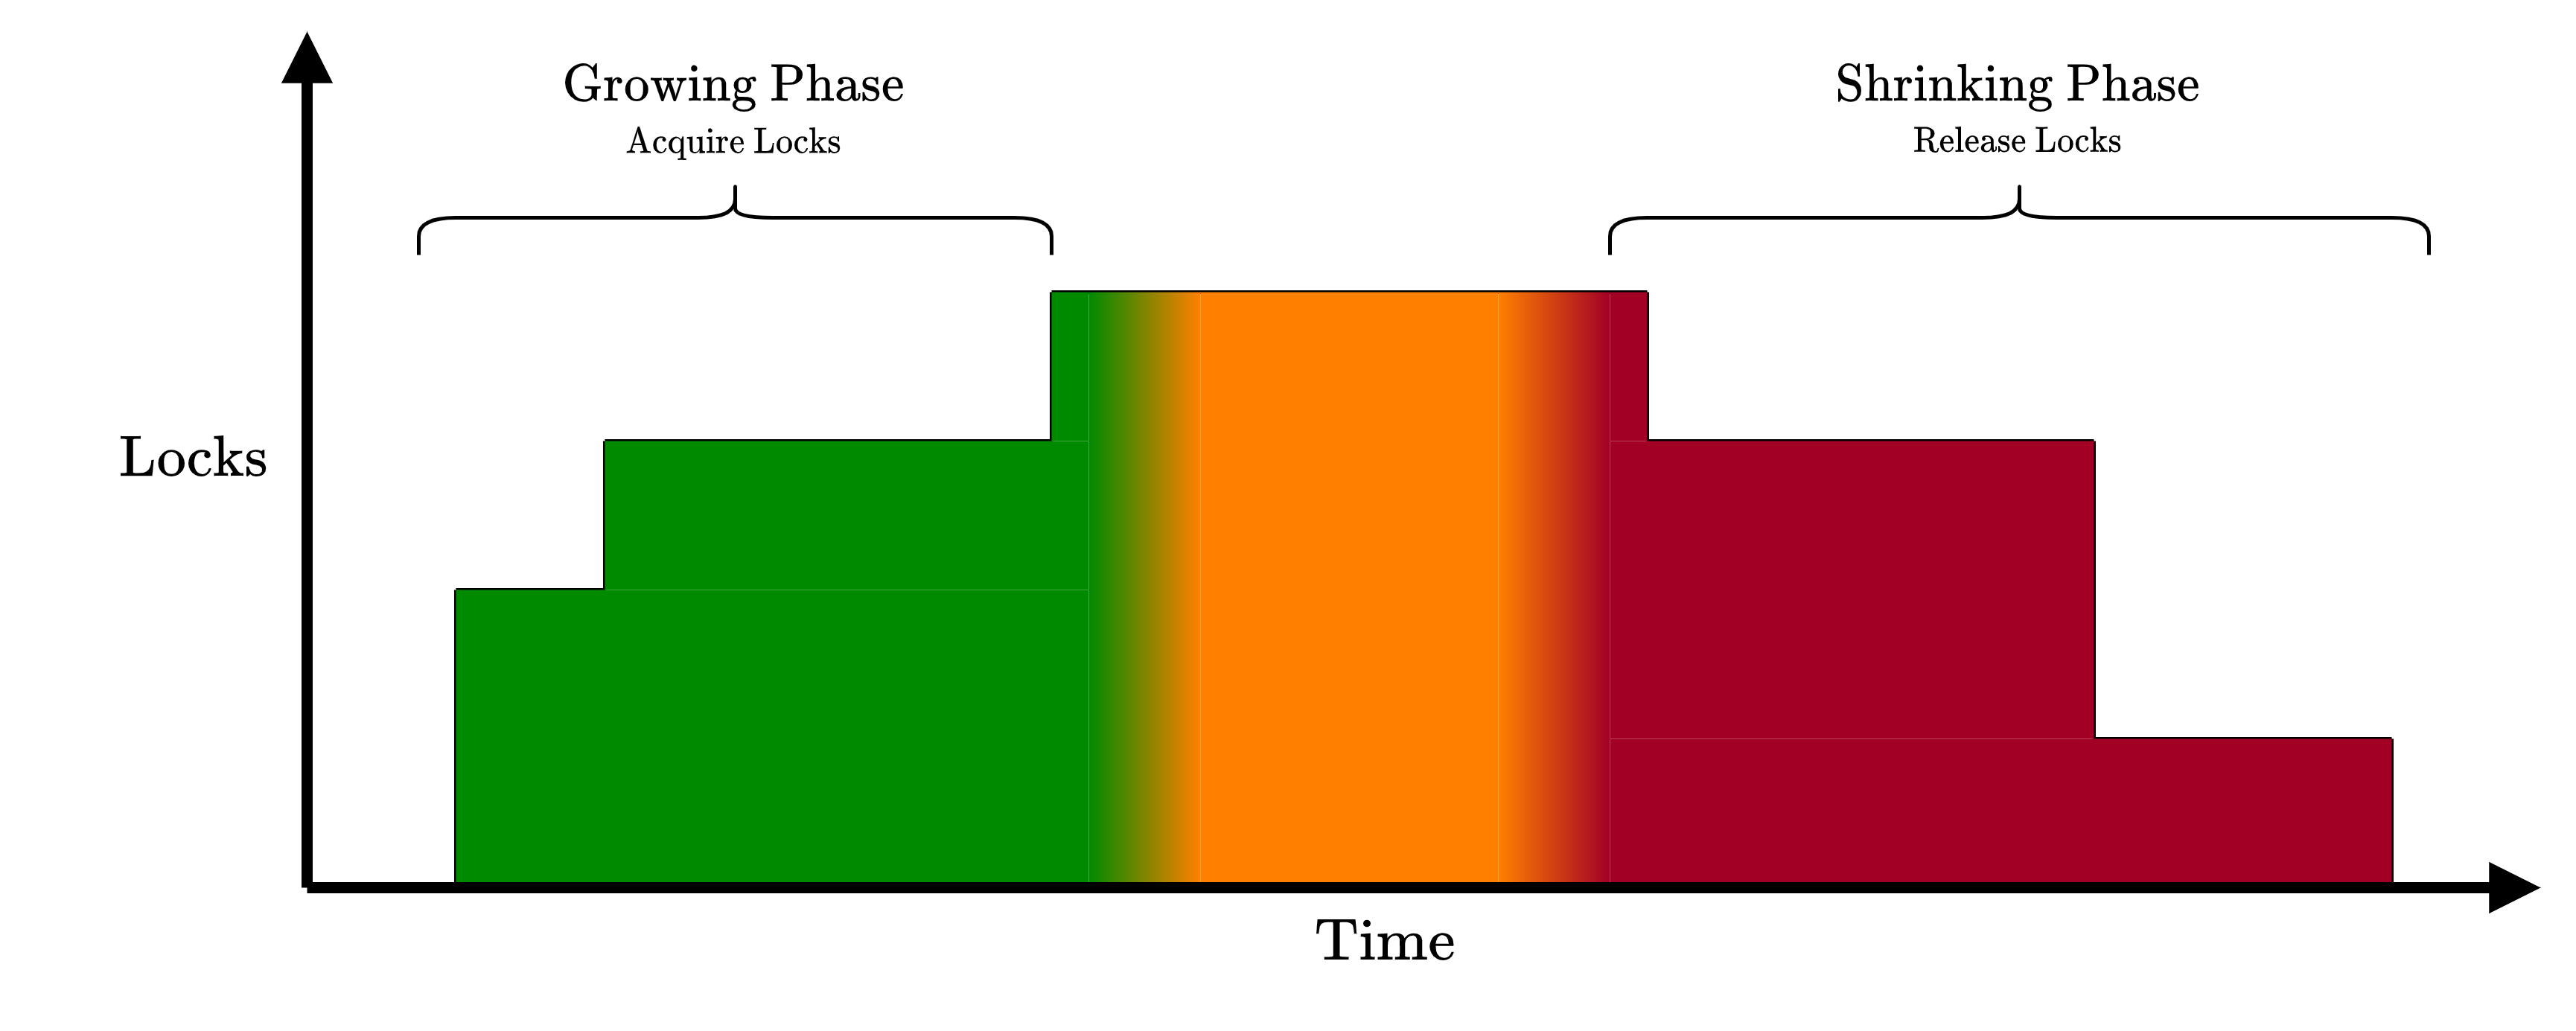
\includegraphics[width=.9\textwidth]{transactions/images/2_phase_locking.drawio.png}
\end{center}
\begin{itemize}
    \item Transaction acquires locks required in \textit{growth phase}, and releases in \textit{shrinking phase}.
    \item Acquires locks on objects before reading/writing.
\end{itemize}
\subsubsection{Deadlocks}
Deadlocks must be prevented, this can be achieved in several ways:
\begin{itemize}
    \item Acquire locks in a global order $\to$ we cannot know which locks a query may need ahead of time.
    \item Complete a \textit{dry-run} to determine required locks, before then accessing in global order $\to$ transactions may occur between \textit{dry-run} and run, and hence change the set of locks required.
    \item Timeouts: Locks safe for a predefined time, after this if another transaction acquires the lock, it aborts the holding transaction.
    \item Cycle Detection: At regular intervals, inspect locks, waiters and holders to compute a graph, and abort transactions (usually youngest) to remove cycles.
\end{itemize}

\subsubsection{Lock Manager}
\begin{center}
    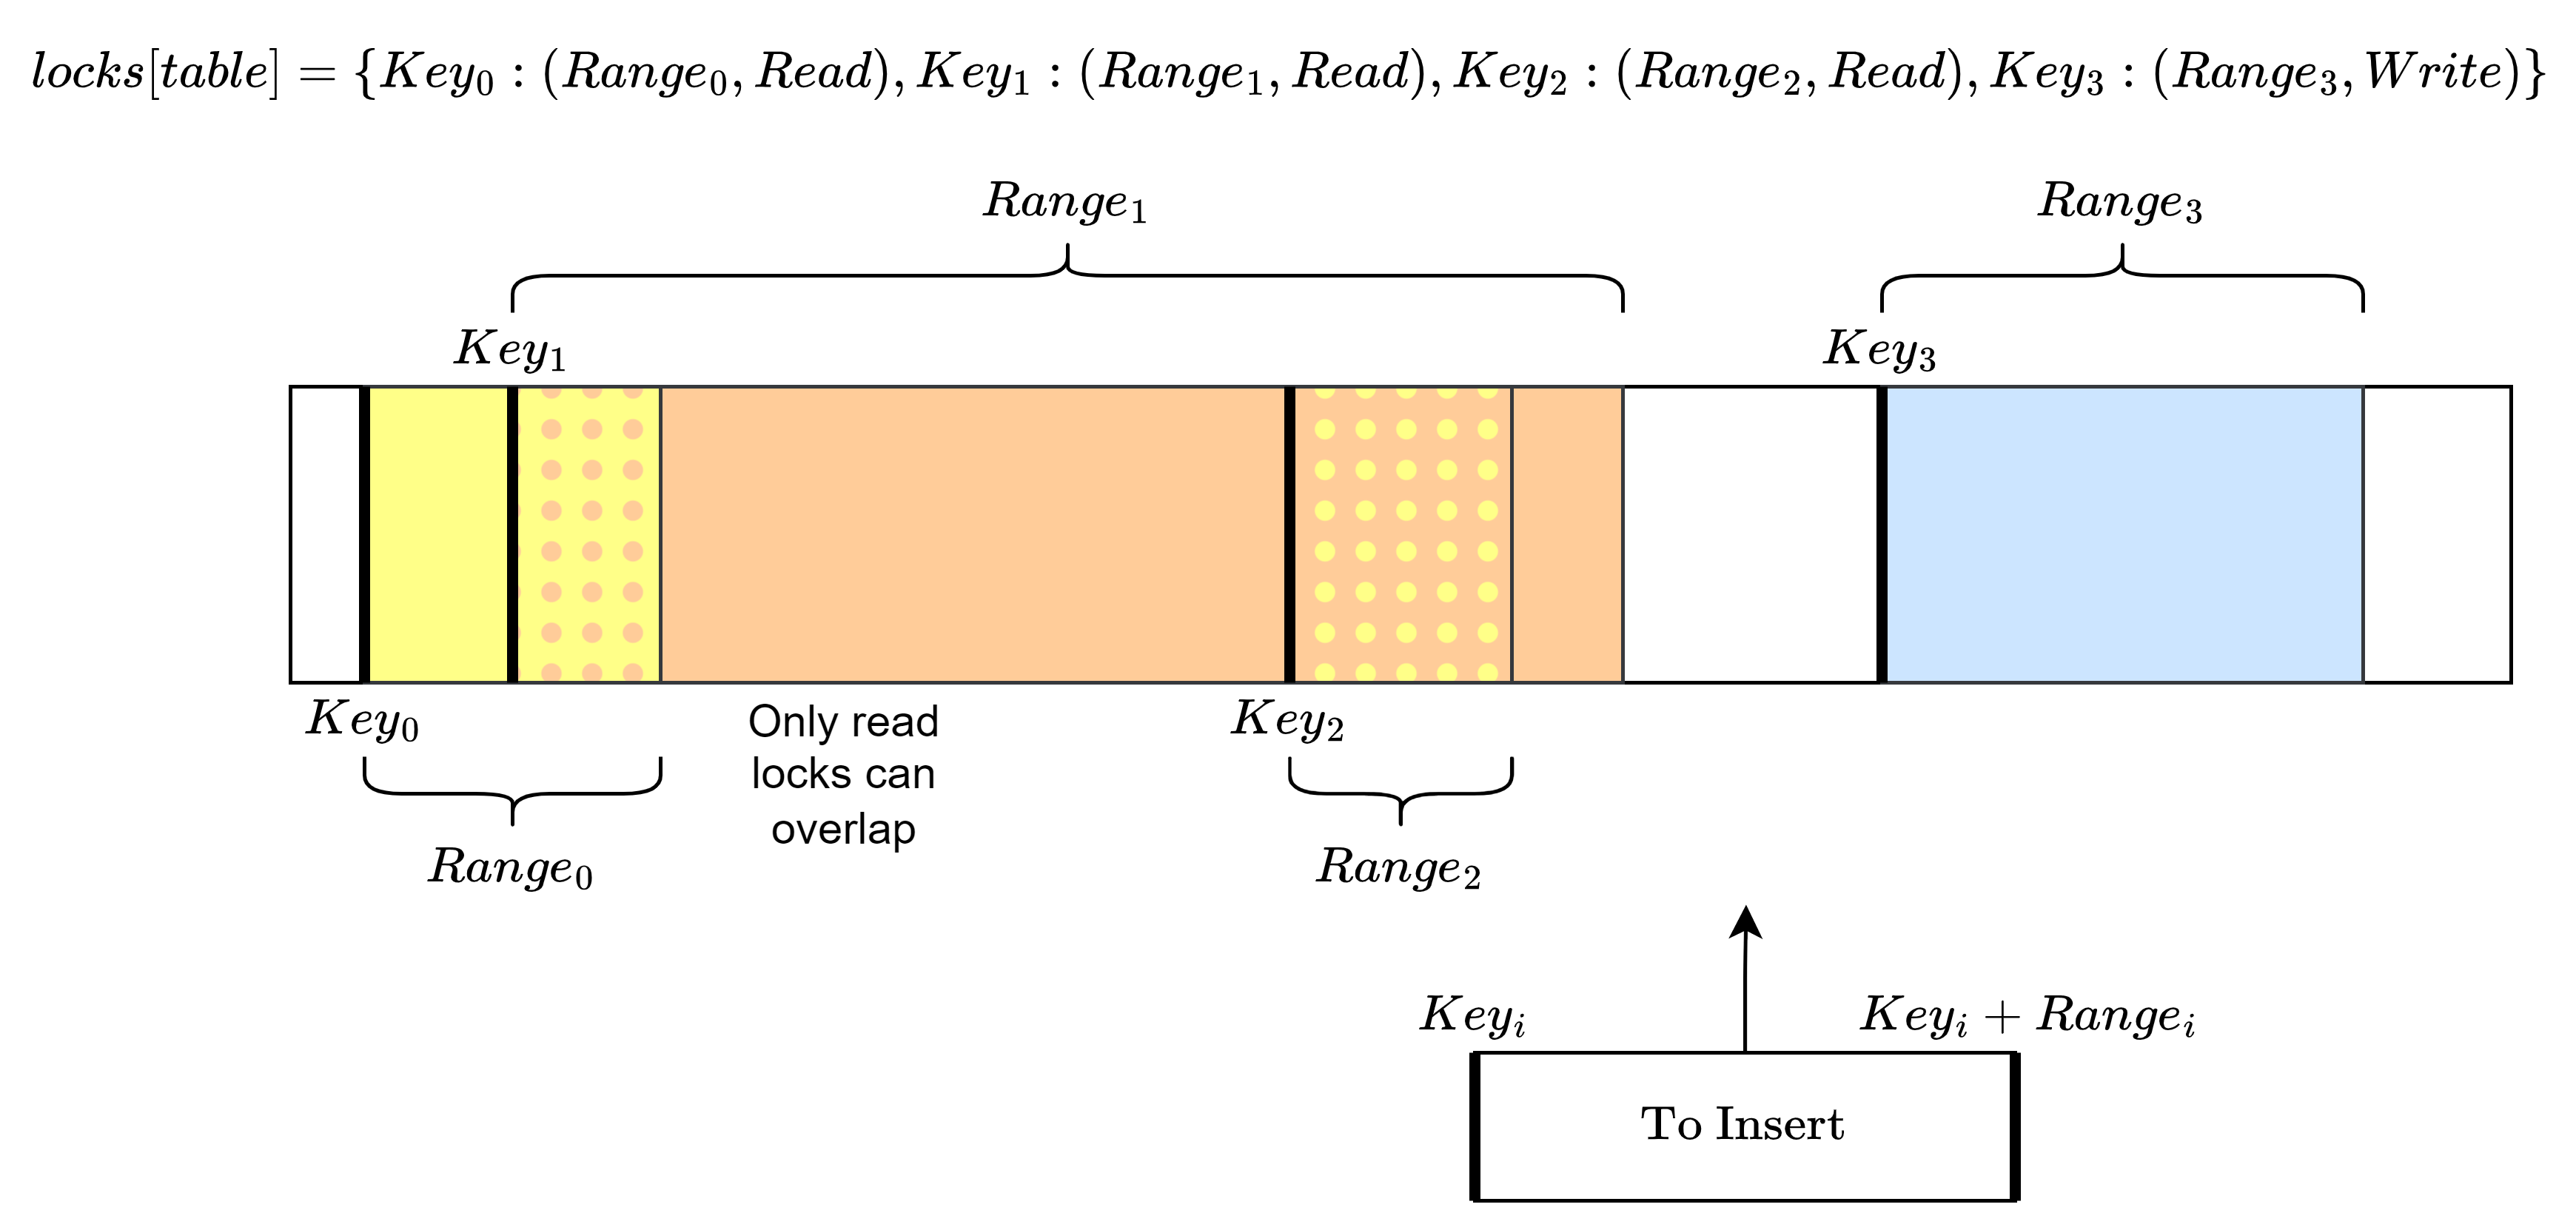
\includegraphics[width=.8\textwidth]{transactions/images/lock_manager_ranges.drawio.png}
\end{center}
Manages the locking of ranges within tables as either read or write.
\begin{itemize}
    \item Checks for conflicts in overlapping ranges
    \item Ensures locks are released properly
\end{itemize}

\unfinished

\begin{tabbox}{prosbox}
    \textbf{Serializable} & \textit{2PL} ensures realizability (and hence no anomalies). \\
\end{tabbox}
\begin{tabbox}{consbox}
    \textbf{Deadlock Detection} & Can be expensive to avoid \& complex to implement. \\
    \textbf{Mutual Exclusion} & Ranges are locked, so cannot read \& write, or write \& write in parallel. \\
\end{tabbox}

\subsection{Timestamp Ordering}
Each tuple is timestamped for \textit{last read} and \textit{last write}, and every transaction is timestamped at the start of execution.
\begin{center}
    \begin{tabular}{l p{.7\textwidth}}
        \textbf{Read} & Check tuple read timestamp (if newer than transaction timestamp abort), set read timestamp to transaction timestamp. \\
        \textbf{Write} & Check tuple write timestamp (if newer than transaction timestamp abort), set write timestamp to transaction timestamp. \\
    \end{tabular}
\end{center}

\subsection{Optimistic Concurrency Control (OCC)}
Run transactions without locks, buffering reads, inserts and updates until commit. At commit check if the database is unmodified (if not then abort) and apply with locks.
\begin{itemize}
    \item The simplest multiversion concurrency scheme.
    \item Can use a timestamp to determine when rows have been changed.
\end{itemize}

\begin{tabbox}{prosbox}
    \textbf{Few Conflicts} & Performant when the number of conflicts is low (e.g analytics database with few updates). \\
\end{tabbox}

\subsection{Multi-Version Concurrency Control (MVCC)}
Store different versions of the tuple at different timestamps to allow a transaction to use old committed data, as new committed data is written to the \textit{same} rows.
\begin{itemize}
    \item Transactions use tuples that have the latest timestamp less than the transaction's start.
    \item Timestamps can be stored with tuples, or separately. Table structure needs to allow for multiple versions of the same \textit{row} (e.g append new rows into one large table, or table entries are lists of rows etc.)
\end{itemize}

\begin{tabbox}{prosbox}
    \textbf{Many Conflicts} & Performs better than other concurrency control schemes when conflicts are frequent (conflicts do not force transactions to wait). \\
    \textbf{Time travel} & Multiple versions of tuples allow for quick rollbacks, to inspect recent past values for rows. \\
\end{tabbox}
